\documentclass[12pt, a4paper]{article}
\usepackage[utf8]{inputenc}
\usepackage[russian]{babel}
\usepackage[T2A]{fontenc}
\usepackage{amsfonts}
\usepackage{amsmath}
\usepackage{indentfirst}
\usepackage{amsthm}
\usepackage{algorithm,algpseudocode}
\usepackage{float} 
\DeclareMathOperator*{\argmin}{argmin}
\newtheorem{lemma}{Утверждение}[section]

\usepackage[left=2cm,right=1.5cm,top=2cm,bottom=2cm]{geometry}
\linespread{1.25}

\usepackage{graphicx}
\graphicspath{{pictures/}}
\DeclareGraphicsExtensions{.pdf,.png,.jpg}

\begin{document}
\pagestyle{empty}

\begin{center}
	ФЕДЕРАЛЬНОЕ ГОСУДАРСТВЕННОЕ БЮДЖЕТНОЕ ОБРАЗОВАТЕЛЬНОЕ\\
	УЧРЕЖДЕНИЕ ВЫСШЕГО ОБРАЗОВАНИЯ\\
	<<МОСКОВСКИЙ ГОСУДАРСТВЕННЫЙ УНИВЕРСИТЕТ\\
	имени М.\,В.~ЛОМОНОСОВА>>
\end{center}
\vspace{4pt}
\begin{center}
	МЕХАНИКО-МАТЕМАТИЧЕСКИЙ ФАКУЛЬТЕТ
\end{center}
\vspace{4pt}
\begin{center}
	КАФЕДРА ВЫЧИСЛИТЕЛЬНОЙ МАТЕМАТИКИ
\end{center}
\vspace{1cm}
\begin{center}
	ВЫПУСКНАЯ КВАЛИФИКАЦИОННАЯ РАБОТА\\
	специалиста
\end{center}

\begin{center}
	\textbf{ПОСТРОЕНИЕ ОПТИМАЛЬНОГО МАРШРУТА \\
		ПРИ ЗАДАННОЙ МОДЕЛИ ДВИЖЕНИЯ ДРУГИХ \\
		УЧАСТНИКОВ ТРАНСПОРТНОЙ СЕТИ}
\end{center}
\vspace{1cm}
\begin{center}
	\begin{tabular}{p{9cm} l}
		& Выполнил студент $610$ группы\\
		& Разумова Любовь Евгеньевна\\
		& $\phantom{C_n^k=C_n^{n-k}}$\\
		& $\underline{\phantom{\int\limits_a^bf(x)dx=F(b)-F(a)}}$\\
		& подпись студента\\
		& $\phantom{\int\limits_f(z)dz=0}$\\
		& Научный руководитель:\\
		& доктор физико-математических наук \\
		& Афонин Сергей Александрович\\
		& $\phantom{C_n^k=C_n^{n-k}}$\\
		& $\underline{\phantom{\int\limits_a^bf(x)dx=F(b)-F(a)}}$\\
		& подпись научного руководителя\\
	\end{tabular}
\end{center}
\vspace{1cm}
\begin{center}
	Москва\\
	$2022$
\end{center}

\newpage
\pagestyle{plain}
\tableofcontents{}

\newpage	

\section*{Введение}

В данной работе рассматривается задача нахождения наилучшего в смысле временных затрат пути с учетом движения фиксированного количества участников по заданным маршрутам в рамках некоторой модели движения. Под моделью движения понимается некий набор правил, которые задают скоростной режим участника движения в зависимости от его взаимодействия с другими автомобильными транспортными средствами (АТС). Маршруты участников могут пересекаться, что приводит к изменению скорости участников и образованию заторов. Целью работы является проложение оптимального маршрута в условиях возможности возникновения пробок на вариации подходящих путей.

%Одной из подзадач является разработка таких правил, которые были бы близки к естсвественному характеру взаимодействия автомобильных  траснспортных средств (АТС).
%в условиях ограниченности модели дорожной системы.

\if 0
В данной работе рассматривается задача нахождения наилучшего в каком-то смысле пути с учетом движения фиксированного количества участников по заданным ранее маршрутам в условиях ограниченности модели дорожной системы. Новый построенный маршрут должен отвечать выбранному критерию оптимальности среди всевозможных путей на всем временном промежутке, но не обязательно в каждый момент времени. Знание маршрутов изначальных участников помогает определить плотность автомобильного потока на конкретных отрезках пути. Рассматриваемая модель приближена к реальной дорожной системе городов, поэтому на всех ее участках наложены ограничения по вместимости участников и скорости их движения. Такие ограничения влияют на показатели маршрутов участников, такие как итоговое время движения и длину пути. 
\fi

Задачи на транспортную тематику никогда не теряют своей актуальности, в том числе и задача маршрутизации. Сложно найти человека, который в целях сбережения личного времени не пользуется какой-нибудь системой навигации, не говоря уже о сервисах такси, для которых крайне важно минимизировать временные затраты в пути. Однако данная задача решается построением оптмального маршрута с учетом картины заторов на момент составления этого маршрута. Образование заторов --- часто непредсказуемое явление, и пробка может появиться прямо перед нами на участке пути, который при построении маршрута был свободен. Несмотря на то, что время и место заторов сложно предугадать, задачей их прогнозирования занимаются уже долгое время.
% Тема актуальна и в наше время, так как она помогает решать проблему возникновения пробок на дорогах, а также призвана упростить водителям выбор маршрута, который займет у них наименьшее время. 
%Задача имеет практический характер... Проблема пробок в Москве стоит очень остро, ученые решают ее не первый год..

Помимо систем навигации прогнозы загруженности используются для автоматического управления дорожным движением в некоторых городах. Первые прототипы, в которых были применены прогнозы, появились появились в 1998 году в США. А первое пилотное использование системы, «заглядывающей в будущее», началось в 2006 году в Сингапуре в целях заблаговременного предупреждения водителей о дорожных условиях впереди и ценах, взимаемых за пробки в данный момент. Среди наших соотечественников задачей прогнозирования занимаются разработчики Яндекс.Пробок. Программисты собирают информацию по трекам движения автомобилей, осуществляют привязку треков к ребрам графа дорожной сети, вычисляют некоторую усредненную скорость на отдельных участках, рисуют карту прогноза дорожной ситуации на ближайший час и в связи с этим предлагают оптимальный по времени путь, а также еще пару альтернативных маршрутов. Сложность сбора информации и построения треков движения состоит в том, что, во-первых, не все пользуются сервисами Яндекса при построении своего маршрута, и во-вторых, в данных постоянно возникают лишние шумы, что приводит к выбросам на графиках, и с таким качеством информации работать очень сложно. Мы же рассматриваем более прозрачную и простую модель, когда все маршруты изначально проложены и известны, и они не меняются с течением времени. Это не умаляет значимости и важности поставленной нами задачи. Путем моделирования движения можно получить более точные результаты, идеи в дальнейшем могут развиваться и открывать новые возможности для более широкой задачи, например, как у Яндекса. 
%Стоит отметить, что на конференции Yet another Conference в 2012 году разработчики впервые поделились результатами о применении машинного обучения в прогнозировании пробок. До этого пользователи могли пользоваться только картой пробок на текущий момент и историческим прогнозом на основе статистики.  
 Также стоит отметить, что разработчики Яндекс.Пробок используют статистические методы и машинное обучение в качестве инструмента для решения своих задач, мы же подойдем к вопросу с другой стороны и применим другие алгоритмы.
  
  Отдельное внимание стоит уделить построению математической модели для описания движения АТС. Существует множество различных моделей движения, например, в модели Лайтхилла–Уизема (Уитема)–Ричардса (LWR) \cite{hydro_1}, \cite{hydro_2} однополосный транспортный поток рассматривается как поток одномерной сжимаемой жидкости. Модель LWR была первой среди гидродинамических. Теория развивалась и появлялись новые модели, такие как модель Танака \cite{Tanaka} --- LWR-модель, где плотность потока зависит от некоторой дистанции видимости, зависящей от скорости потока. В микроскопической модели Ньюэлла \cite{Newwell} постулируется, что для каждого водителя существует безопасная скорость движения, зависящая от дистанции до лидера. 
   В своей работе мы позаимствовали деление моделей движения на макро- и микроскопические \cite{book} и разработали свои модели взаимодействия участников движения.


Задачи, которые мы ставили перед собой в рамках выбранной темы дипломной работы: формальная постановка задачи, анализ полученных ранее результатов в этой теме, разработка модели движения, которая была бы близка к естественному характеру взаимодействия АТС, исследование примененимости различных алгоритмов к решению поставленной задачи. Методом исследования является моделирование движения.

%Основа нашей задачи - нахождение наилучшего пути в условиях изменчивости плотности и скорости дорожного потока на участках в заисимости от времени.

В первом разделе вы сможете ознакомиться с определением модели движения как некоторого автомата и деталями поставленной задачи. Во втором разделе будет представлена классификация моделей движения с примерами. Далее мы опишем процесс моделирования произвольной дорожной ситуации. Четвердый раздел посвящен описанию алгоритмов и исследованию их примененимости. В завершении поделимся результатами проделанной работы, оценим их качество и сделаем выводы.




\newpage
\section{Постановка задачи}

Пусть задан ориентированный \textit{граф дорожной сети} $ G (V, E, l)$ таким образом, что вершины $ v \in V$ осуществляют роль перекрестков, а ребра $e \in E$ - роль дорог. Каждое ребро имеет длину, т.е. задана функция $l : E \rightarrow \mathbb {R} $. Также мы говорим, что задана некоторая модель движения.
%Формализуем понятие модели движения, упомянутое в постановке задачи.  Обратимся к теории автоматов и с ее помощью попробуем описать правила движения АТС.
Обратимся к теории автоматов, чтобы попробовать формализовать подразумеваемые под этим понятием правила движения АТС. Аналогичный подход использовали К.\,Нагель и М.\,Шрекенберг \cite{automat_baza}. В своей работе авторы рассматривают модель клеточных автоматов, которая предполагает разбиение дорог на клетки и использование дискретного времени. Эта идея нашла применение в описании движения физических частиц \cite{automat_phyz}, а также в исследовании пробок на дорогах \cite{automat_jam}. Мы же не будем ограничиваться клеточными автоматами и опишем случай непрерывного движения.

\textit{Моделью движения} АТС назовем $M = \left(n, G, S, F, \{t_i\}_{i = 1}^n, \{\varphi_i\}_{i = 1}^n \right)$, где $n$ - количество участников движения, $G$ --- граф дорожной сети, $S$ --- множество состояний, которые могут принимать участники, $F \subset S$ --- множество заключительных состояний, $t_i: S^n \rightarrow R_{>=0}$ --- функция критического момента движения участника $i$, $\varphi_i: S^n \times \mathbb{R}_{>= 0} \rightarrow S$ --- функция перехода состояния $i$-ого участника в некоторый момент времени $t$. Считаем, что, попав в заключительное состояние, мы не можем его покинуть:
$$\varphi_i (s_1, \dots, s_i, \dots, s_n, t) = s_i, \text{ } s_1, \dots, s_n \in S, \text{ } s_i \in F, \text{ } \forall t \in \mathbb{R}_{\ge 0}.$$
Множество $S$ описывает текущий характер двжиения АТС. Это, в первую очередь, ребро, на котором едет участник, координата на этом ребре, скорость участника и его ускорение, если оно есть.
%Если модель описывает некоторое измение ускорения, то под состоянием $s$ также имеется ввиду текущее ускорение машины.
Подразумевается, что состояния можно разбить на классы, например <<свободное движение>>, <<ожидание>>, <<прибытие>>, <<торможение>>, <<ускорение>> и тд. Функция $t_i$ описывает время, когда участнику необходимо совершить переход из текущего состояния в состояние другого класса. 

Модель движения АТС можно описать некоторой диаграммой, описывающей переходы между классами для каждого участника. Диаграмма представляет собой ориентированный граф, где вершины --- классы состояний, а ребра являются переходами в другое состояние. Метка на ребре --- условие перехода, который осуществляется, если $t =  t_i(s_1, \dots, s_n)$ для некоторого $s_i$ из класса состояний. Непомеченные ребра соответствуют условию $t < t_i(s_1, \dots, s_n)$:
$$\varphi_i (s_1, \dots, s_n, t) = s_i, \text{ } s_1, \dots, s_n \in S, \text{ } 0 \le t < t_i(s_1, \dots, s_n).$$
 Например, правила движения, в которых поведение участника зависит от расстояния, до впереди идущего участника может быть задано следующей диаграммой (см. рис. \ref{ris:example_diag}):
\begin{figure}[H]
	\centering
	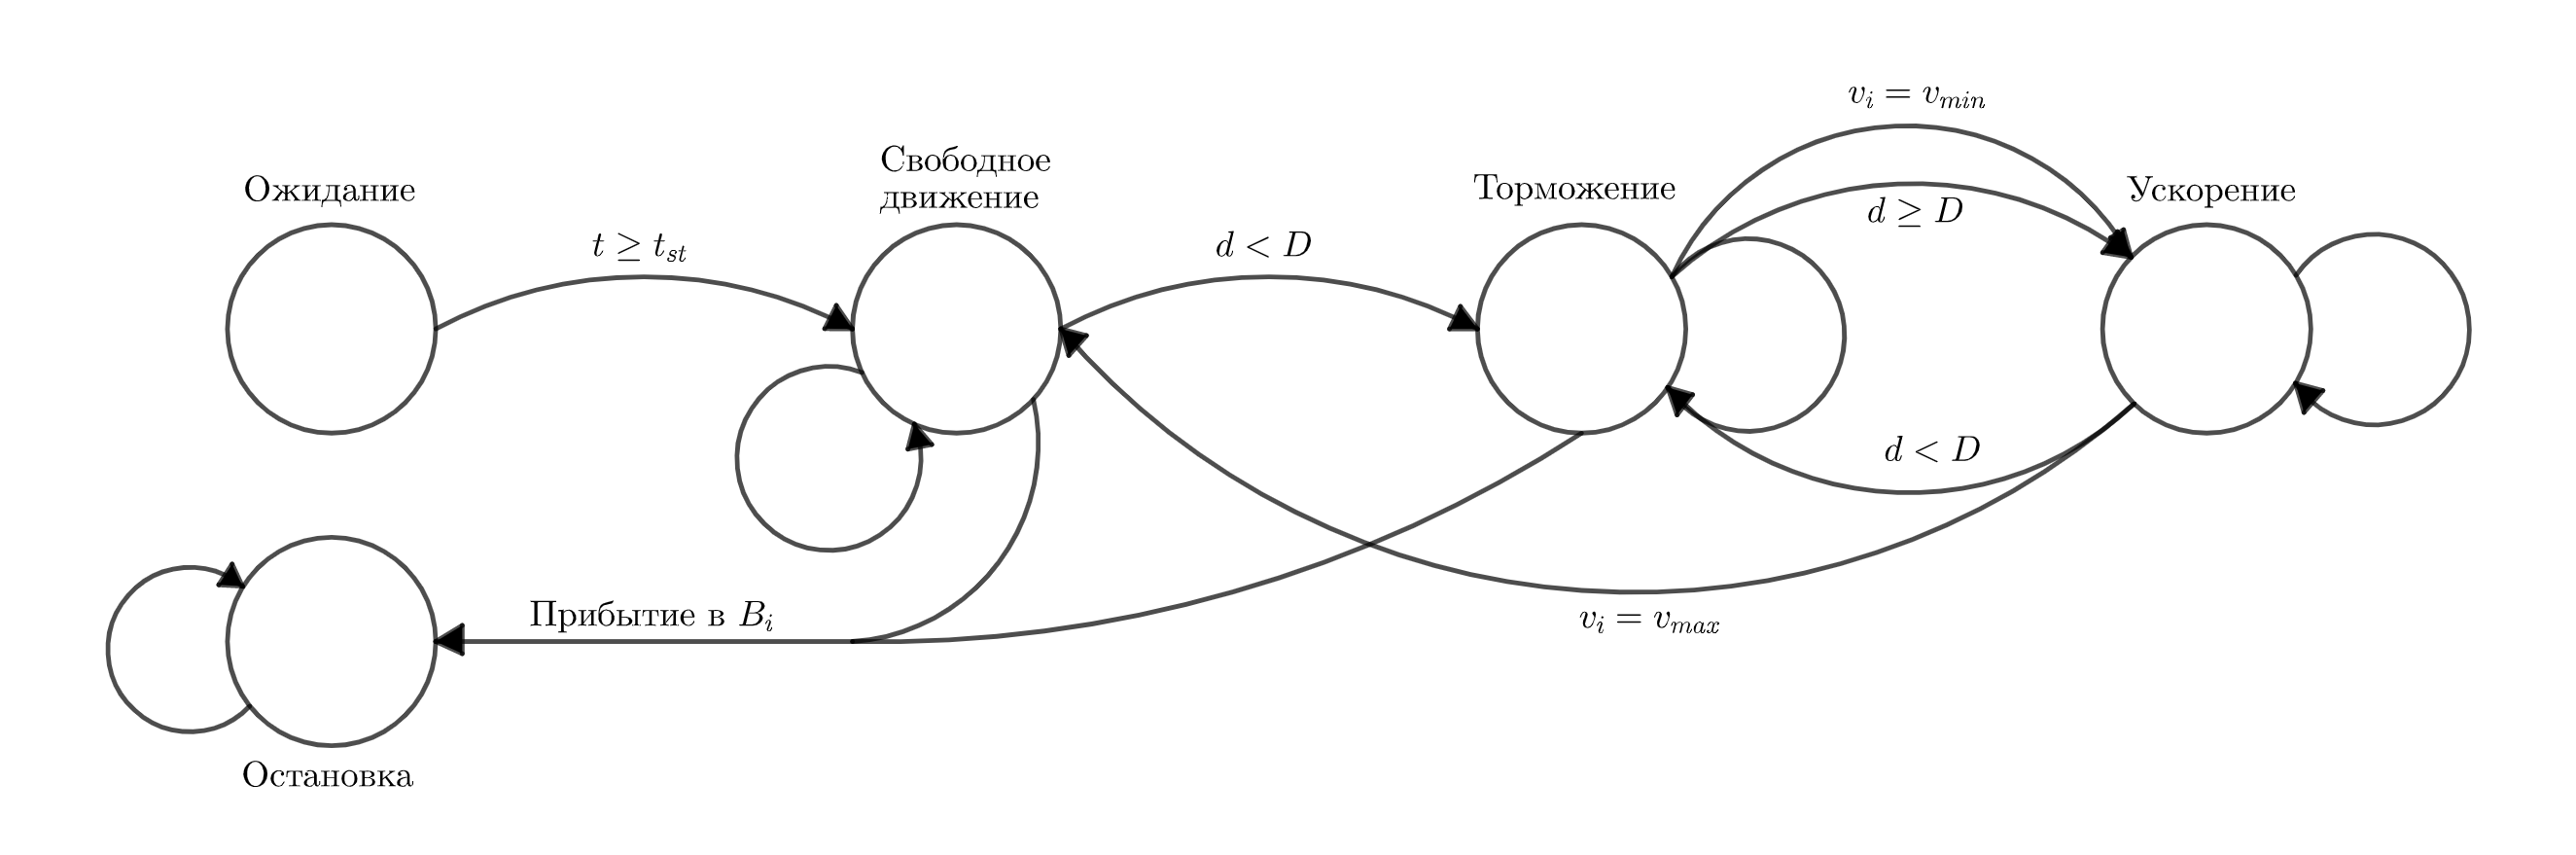
\includegraphics[scale=0.25]{example-gen.png}
	\caption{Диаграмма для $i$-ого участника в модели движения, где $d$~-- расстояние до впереди идущего участника, $D$~-- максимальное расстояние взаимодействия с впереди идущим участником, $v_{max}$~--максимально возможная скорость, $v_{min}$~--минимально возможная скорость, $t_{st}$~-- время старта.}
	\label{ris:example_diag}
\end{figure}

Перейдем от формального определения модели движения непосредственно к постановке задачи.
Пусть имеется $n$ участников, которые движутся по заранее заданным маршрутам:  $ p_i = \langle E^i_{j_1}, E^i_{j_2}, \dots, E^i_{j_{m_i}} \rangle$, $ E^i_{j_k} \in E \quad i = 1, \dots, n$. Добавим к ним $(n+1)$-ого участника, которому нужно добраться из пункта $A$ в пункт $B$, $A, B \in V$. Будем считать, что движение добавленного участника не влияет на движение $n$ участников. Определим $P(A,B)$~-- множество всех простых путей из $A$ в $B$. Модель движения позволяет определить \textit{часть пройденного пути} для каждого АТС в зависимости от движения других участников, т.е. определить непрерывные монотонные функции
\begin{center}
 $x_i(G, p_1, \dots, p_n, p, \cdot ) : \mathbb {R} \rightarrow [0 , 1] $, $i = 1, \dots, n+1$, $p \in P(A, B) $.
\end{center}
Ввиду однозначной определенности последовательности ребер $p_j$ и графа дорожной сети $G$, явную зависимость $x_i$ от данных параметров можно не указывать. 

На множестве путей $P(A,B)$ определим $T(p) = \displaystyle \inf_t \{t : x_{n+1}(p, t) = 1\}$~-- время прибытия $(n+1)$-ого участника в вершину $B$ при движении по маршруту $p$. Требуется найти такой путь $p^* \in P(A, B)$, что $T(p^*)$ - минимальна. Другими словами, для заданной модели движения на графе дорожной сети $G(V, E, l)$ при движении $n$ участников по путям $p_1, \dots, p_n$ требуется найти такой путь $p^*$ из $A$ в $B$, что движение нового участника по этому пути $p^*$ будет \textit{оптимально}, то есть
$$p^* = \argmin_{p \in P(A, B)} T(p).$$

\newpage
\section{Модели движения}

В первую очередь для решения задачи, нужно конкретизировать модели движения. Рассмотрим те из них, в которых изменения скорости участников базируются только на количестве участников на ребре в момент времени $t$. Назовем такие модели \textit{макроскопическими}, а все остальные --- \textit{микроскопическими}. 

\if 0
%Нас интересует точное решение, поэтому промоделируем движение $n$ участников, чтобы в каждый момент времени были известны функции $x_i(t)$. 
Поведение движения АТС в нашей постановке задачи определяется некоторой системой правил. Представим примеры таких приавил, которые описывают естественный, близкий к реальности характер движения автомобилей.

Говоря о поведении движения автомобилей, мы имеем в виду изменение их скоростей в зависимости от ситуации на дороге. Для каждого АТС введем функцию \textit{скорости} \\ ${v_i(t) : \mathbb {R}_+ \rightarrow \mathbb {R}_+}$.  Обозначим через $v_m \in \mathbb {R}$ максимально возможную скорость, или \textit{скорость свободного движения}: $v_i(t) \leq v_m, \forall t \in \mathbb {R}, i = 1, \dots, n+1$.
\fi


\subsection{Макроскопические модели}


При движении $n$ участников макроскопические модели можно параметризовать набором действительных чисел $v_1, \dots, v_n$, где $v_k$~-- скорость при $k$ участниках на ребре. Множество состояний в макроскопических моделях движения можно разбить на $n$ классов по количеству участников на ребре (см. рис. \ref{ris:macro_diag}).  Общее количество всех возможных переходов между классами состояний для $i$~--ого участника составит $n(n-1) + 2n$.

\begin{figure}[H]
	\centering
	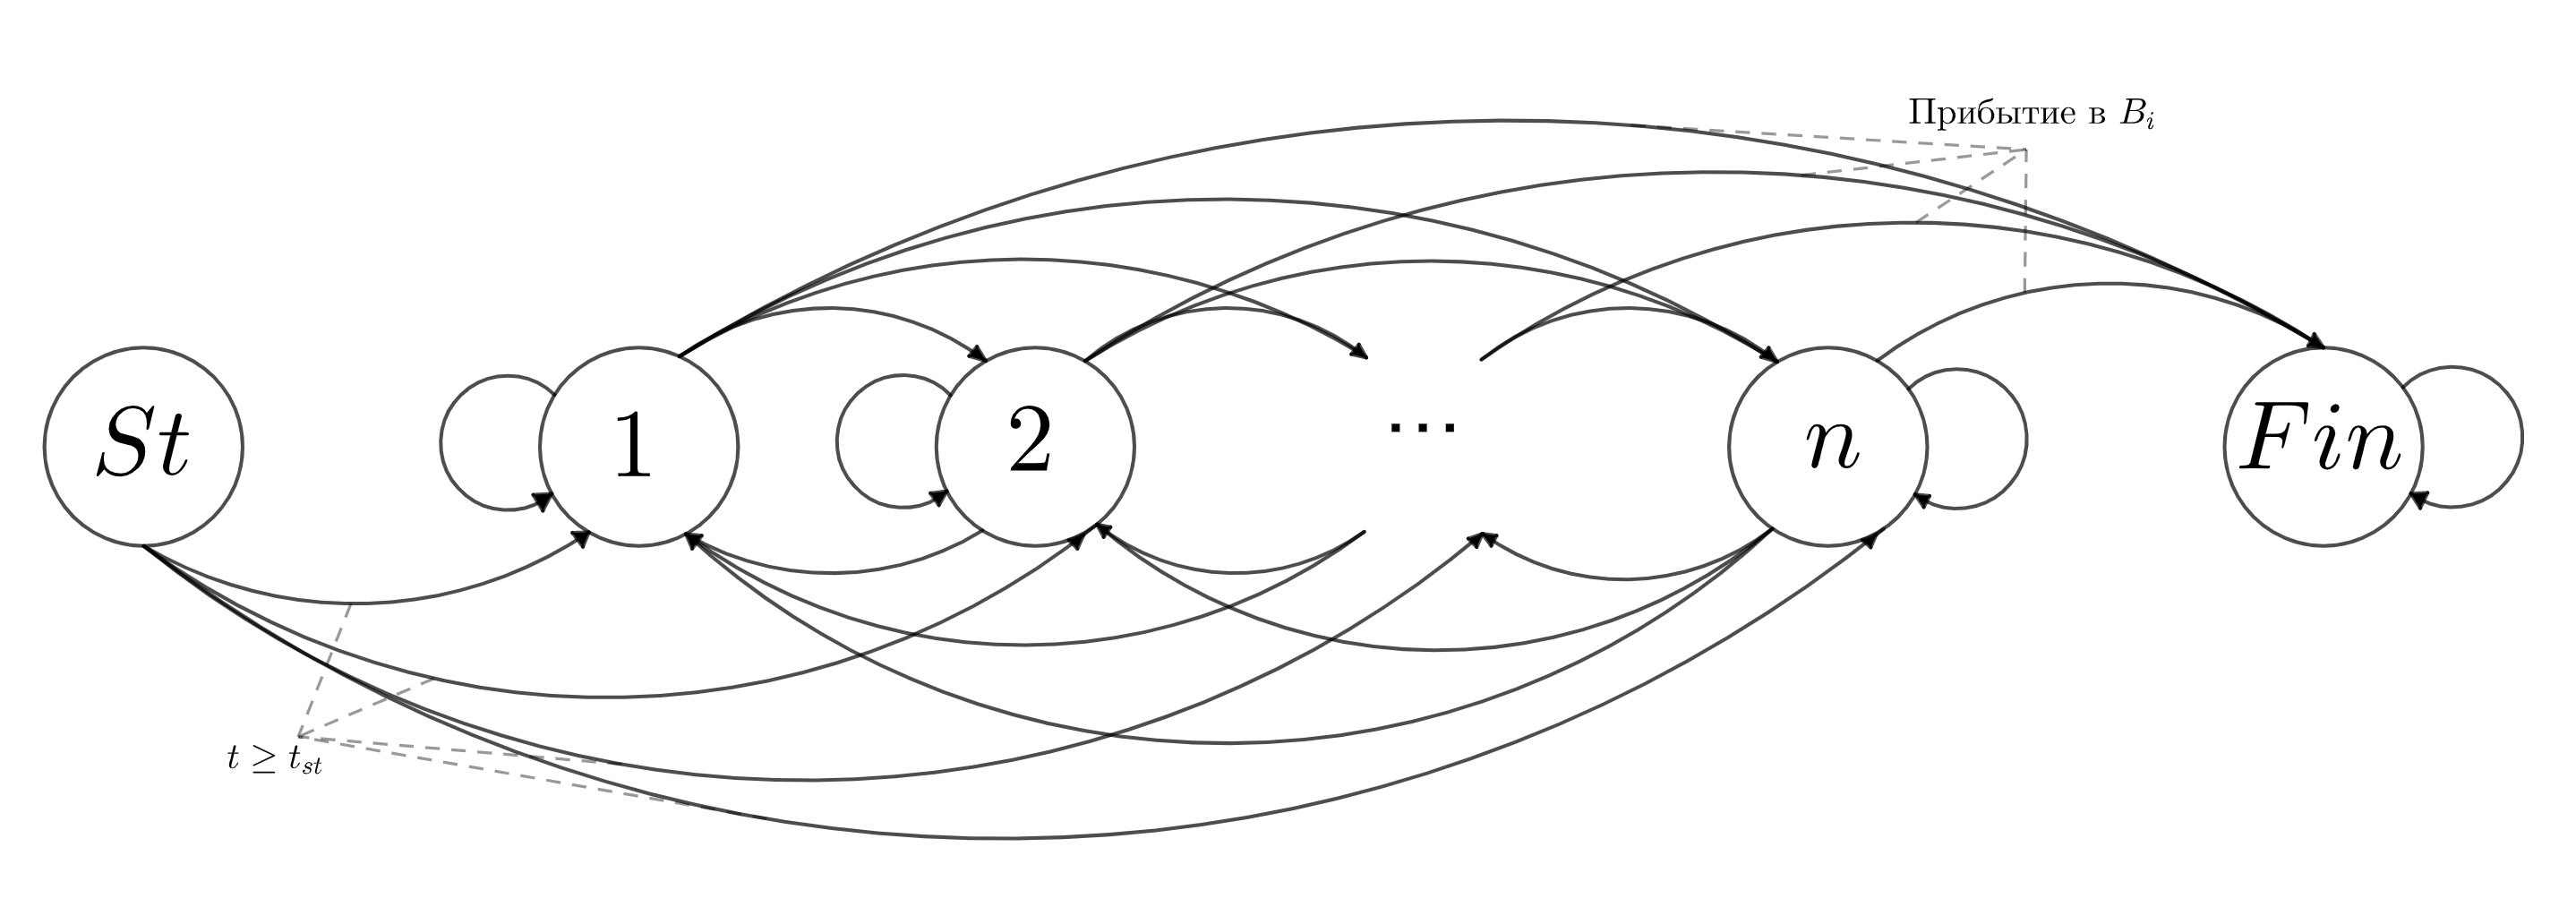
\includegraphics[scale=0.2]{Macro-gen.png}
	\caption{Диаграмма для $i$-ого участника в макроскопических моделях движения}
	\label{ris:macro_diag}
\end{figure}
Пусть $n_i$~-- количество участников на ребре $e_i$, на котором находится участник $i$. Переходы из состояния $k$ в состояние $m$ осуществляются при выполнении сразу двух условий: $n_i \neq k$ и $n_i = m$. При этом критический момент для $i$~--ого участника наступает, когда какой-либо участник въезжает на ребро $e_i$ или съезжает с него. Так, если $\chi_i$~-- часть пройденного $i$-ым участником ребра $e_i$, то 
$$t_i = min \left\{\frac{l(e_j)\left(1-\chi_j\right)}{v_{n_j}} \; \bigg| \; j = 1, \dots, n; \; e_j = e_i \text{ или следующее за } e_j \text{ ребро в } p_j \text{ это } e_i\right\}.$$

Для того, чтобы критические моменты $t_i, \: i = 1, \dots, n$ были определены, макроскопические модели требуют положительности скоростей $v_i, \: i = 1, \dots, n$. Условие $v_i \ge v_{min} > 0, \: i = 1, \dots, n$ обеспечивает достижимость переходов в другие классы состояний:
$$t_i < T_i = \frac{max\{l(e_i) \: | \: e_i \in p_i\}}{v_{min}}.$$
Количество таких переходов для участника $i$ будет ограничено количеством ребер в пути $p_i$, из чего можно сделать вывод, что все заключительные состояния достижимы.


  Примером такой модели может послужить набор $v_k = \frac{v_{max}}{k}$ для $k$ участников на ребре, $k \in \{1, \dots, n\}$, где $v_{max}$~-- заданная максимальная скорость. 

\subsection{Микроскопические модели}

Микроскопические модели, в отличие от макроскопических, предполагают другой набор другие зависимости скоростей.
Опишем модель \textit{следования за лидером}~-- модель, в которой поведение движения участника зависит от расстояния до впереди идущего АТС. 

Пусть заданы максимальная $v_{max} > 0$ и минимальная $v_{min} > 0$ скорости участников, и ускорение $a = const, \: a > 0$, которое позволяет разгоняться от $v_{min}$ до $v_{max}$. Будем считать, что участники подчиняются следующему правилу:
% должны соблюдать \textit{безопасное расстояние} $l$~---
оказавшись на расстоянии $d \leq l, \: l > 0$, которое мы будем называть \textit{дистанцией торможения}, до лидера, участник
 %не может к нему приближаться. В этом случае участник
  мгновенно сбрасывает свою скорость до минимальной и продолжает движение с постоянной скоростью, пока не отдалится от лидера на \textit{безопасное расстояние} $D > l$. Оказавшись на расстоянии $D$ до лидера, участник с минимальной скоростью может перейти к равноускоренному движению. Диаграмма такой модели движения представлена на рис. \ref{ris:micro_diag}.
  % Расстояние $l$ будем называть \textit{дистанцией приближения}. 

\if 0
 Введем понятие \textit{дистанции видимости} или \textit{зона видимости} $D$~--- расстояние, на котором участник начинает взаимодействовать с впереди идущим лидером и в связи с этим менять свой характер движения. Также будем считать, что участники должны соблюдать \textit{безопасное расстояние} $l < D$~--- оказавшись на расстоянии $d \leq l$ до лидера, участник не может к нему приближаться. Увеличивать дистанцию между участниками позволит ускорение, которое мы зададим некоторой положительной константой.


Пусть $i$~-ый и $(i+1)$~-ый участники, лидер и следующий за ним соотвественно, оказались в момент времени $t$ на расстоянии $d$ относительно друг друга со скоростями $v_i$ и $v_{i+1}$. Опишем характер их движения.


\begin{enumerate}
	\item $d \ge D $
	\begin{enumerate}
		\item $v_{i+1} = v_{max} \Rightarrow a_{i+1} = 0$, продолжаем ехать с максимальной скоростью.
		\item $v_{i+1} < v_{max} \Rightarrow a_{i+1} = a_+$ на время $t = \frac{v_{max}-v_{i+1}}{a_+}$, после чего $v_{i+1} = v_{max}, a_{i+1} = 0$
	\end{enumerate}	
	\item $d \leq l \Rightarrow v_{i+1} = 0$
	\item $l < d < D $
	\begin{enumerate}
	\item $v_{i+1} \leq v_i$
		\begin{enumerate}
			\item $a_i = 0$, т.е. его движение равномерно, это может быть только в 2-х случаях:
			\begin{enumerate}
				\item $v_i = v_{max} \Rightarrow a_{i+1} = a_+$ на время $t = \frac{v_{max}-v_{i+1}}{a_+}$, после чего $v_{i+1} = v_{max}, a_{i+1} = 0$
				\item $v_i = 0$, едем время $t = \frac{d-l}{v_{i+1}}$, не меняя скорость, после чего останавливаемся, $v_{i+1} = 0$.
			\end{enumerate}	
			\item $a_i \neq 0 \Rightarrow a_{i+1} = a_i$ 
		\end{enumerate}
	\item $v_{i+1} > v_i$ 
	\begin{enumerate}
		\item $a_i = a_+ \Rightarrow a_{i+1} = a_-$ до момента, когда $v_i + a_it = v_{i+1} + a_{i+1}t$ или $v_{i+1}$ станет $0$, т.е. до $t = min\left(\frac{2Dl(v_{i+1}-vi)}{v^2_{max}(l+D)}, \frac{2lv_{i+1}}{v^2_{max}}\right)$,  после чего $a_{i+1} = a_i = a_+$. 
		\item $a_i = a_- \Rightarrow a_{i+1} = a_i = a_-$.
	\end{enumerate}	
	\end{enumerate}
\end{enumerate}

\fi
\begin{figure}[H]
	\centering
	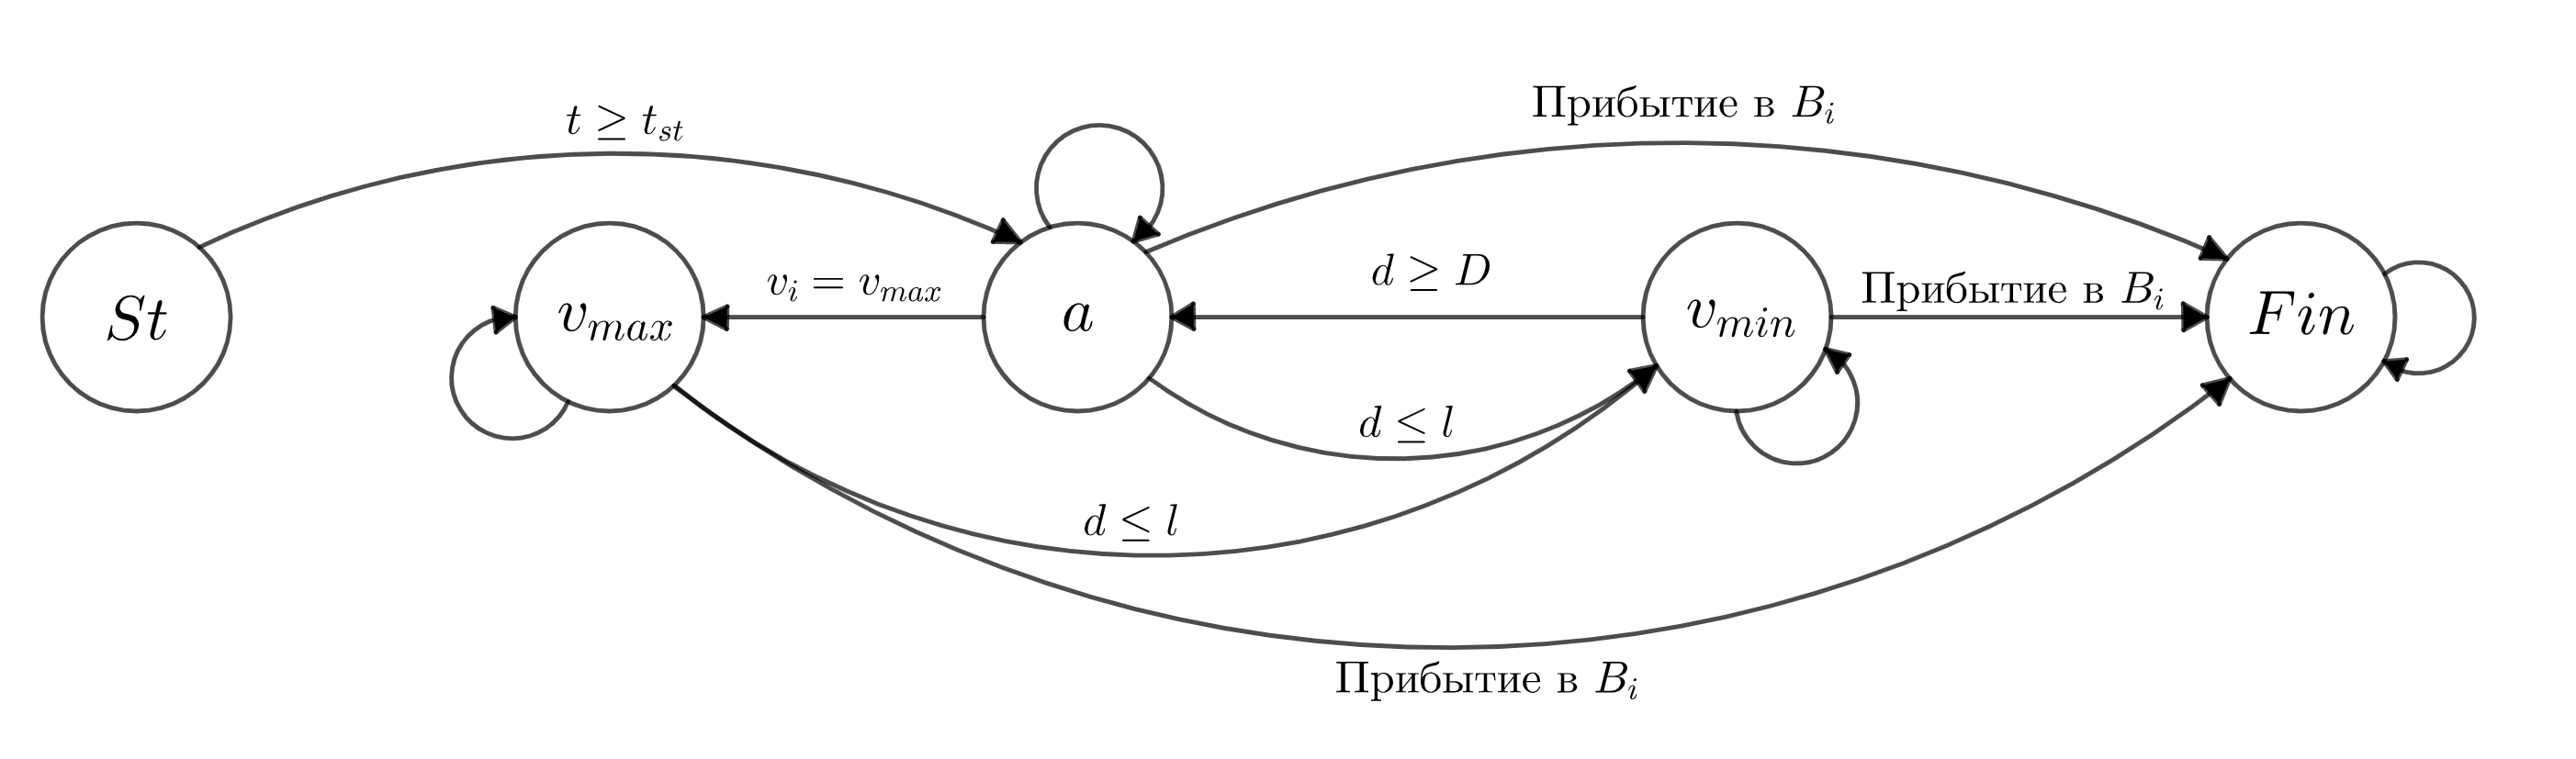
\includegraphics[scale=0.2]{Micro-gen.png}
	\caption{Диаграмма для $i$-ого участника в модели следования за лидером}
	\label{ris:micro_diag}
\end{figure}
\newpage
\section{Моделирование}

%Под моделированием будем понимать воспроизведение движения всех АТС по установленным правилам.
Под моделированием будем понимать воспроизведение движения $n+1$ участника, движущихся по путям $p_1, \dots, p_n, p, \; p \in P(A, B)$ в модели движения $M = M(p_1, \dots, p_n, p)$.
Рассмотрим алгоритм нахождения времени, затраченного $n+1$-ым участником на путь $p$.

\begin{algorithm}[H]
	\caption{Моделирование движения участников}
	\label{alg:modeling}
	{\bf {Input:}} количество участников $n+1$, граф дорожной сети $G$, модель движения $M = M(p_1, \dots, p_n, p)$, набор начальных состояний $s^{\circ}_1, \dots, s^{\circ}_{n+1}$\\
	{\bf {Output:}} $T(p)$\\
	{\bf {Data:}} текущее время $t$, критический момент движения $i$-ого участника $t^*_i$, критический момент $t^*$
	\begin{algorithmic}[1]
		\State $t = 0$
		\For{$i = 1, \ldots, n+1$}
		\State $s_i \gets s^{\circ}_i$
		\EndFor
		\While{$ s_{n+1} \notin F$}
		\For{$i = 1, \ldots, n+1$}
		\State $t^*_i \gets t_i(s_1, \dots, s_{n+1})$ 
		\EndFor
		\State $t^* \gets min \left(t^*_1, \dots, t^*_{n+1} \right)$
		\For{$i = 1, \ldots, n+1$}
		\State $s_i \gets \varphi_i(s_1, \dots, s_{n+1}, t^*)$
		\EndFor
		\State $t \gets t^*$
		\EndWhile
		\State $T(p) \gets t$
	\end{algorithmic}
\end{algorithm}

\if 0

 Рассмотрим 2 различных способа моделирования с $(n+1)$-ым участником: 
\begin{enumerate}
	\item он влияет на движение $n$ участников и вследствие на самого себя;
	\item движение $n$ участников не зависит от добавленного АТС.
\end{enumerate}

\subsection{Независимость движения участников от добавленного АТС}
\subsection{Взаимосвязь движений нового участника и группы АТС}

\fi
\newpage
\section{Поиск оптимального пути}

Отметим, что количество путей конечно, поэтому первое, что приходит на ум в качестве решения, это перебор всех возможных путей и нахождение подходящего по затраченному времени. Посчитаем сложность этого алгоритма и сделаем вывод о его использовании в нашей задаче на практике.

\subsection{Перебор. Сложность}
Чтобы узнать, применим ли перебор в нашем случае, посчитаем сложность нахождения кратчайшего пути среди множества всех простых путей из $A$ в $B$. Пусть $S_M(p)$~-- сложность моделирования, т.е. нахождения функции $x^p_{n+1}(t)$, при выборе пути $p$. Тогда сложность перебора
\begin{center}
 $S = \sum\limits_{p \in P(A,B)} S_M(p) = \vert P(A,B) \vert * \overline S_M$, где $\overline S_M$~-- средняя сложность.
\end{center}
Заметим, что $ S $ растет при увеличении количества возможных путей. Так, в полном графе на $\vert V \vert$ вершинах получим $S = 2^{|V|-2} * \overline S_M$.

В качестве примера можем рассмотерть также регулярный граф-решетку на $\mathbb {R}^2$ и на нем оценить снизу сложность поиска пути с минимальными тратами. Пусть точки $A$ и $B$ имеют координаты $(a_1, a_2)$ и $(b_1, b_2)$ соответственно. Тогда количество путей минимальной длины в метрике Манхэтенна будет составлять $C^{|a_1-b_1|}_{|a_1-b_1| + |a_2-b_2|}$. Понятно, что путей $|P(A,B)|$ в таком графе гораздо больше. Таким образом, получаем оценку снизу для регулярного решеточного графа

\begin{center}
	$C^{|a_1-b_1|}_{|a_1-b_1| + |a_2-b_2|} * \overline S_M  \leq  \vert P(A,B) \vert * \overline S_M = S$.
\end{center}

Например, в решетке-квадрате со стороной $m$ при движении из угловой точки по диагонали в угловую точку напротив количество путей минимальной длины составит $C^m_{2m} = \frac{(2m)!}{m!m!} $. По формуле Стирлинга
\begin{center}
 $ C^m_{2m} = \frac{\sqrt{2\pi(2m)} \left( \frac{2m}{\exp} \right)^{2m}}{\left(\sqrt{2\pi m} \left( \frac{m}{\exp} \right)^m \right)  \left(\sqrt{2\pi m} \left( \frac{m}{\exp} \right)^m \right)} = \frac{2\sqrt{\pi m} \left( \frac{2m}{\exp} \right)^{2m}}{2\pi m \left( \frac{m}{\exp} \right)^{2m}} = \frac{2^{2m}}{\sqrt{\pi m}}$.
\end{center}
Понятно, что при увеличении $m$, количество путей экспоненциально растет.

С помощью перебора можно находить кратчайшие пути быстро, если $|P(A,B)|$ не велико. Однако изначально наша задача была сформулирована в терминах дорожной сети и предполагала графы с достаточно большим количеством вершин и ребер, что влияет на количество маршрутов для заданных точек. Таким образом, можно сделать вывод, что в общем случае перебор путей в нашей задаче на практике не применим.

\newpage
\subsection{Альтернативный подход к решению}


Рассмотрим вспомогательную задачу. Пусть на каждом ребре $e \in E$ графа $G(V, E)$ определена функция \textit{временных затрат} $\phi_e(t) : \mathbb {R}_+ \rightarrow \mathbb {R}_+$. Если мы оказались в начальной вершине ребра $e$ в момент времени $t$, то время преодоления ребра будет равняться $\phi_e(t)$. Рассмотрим путь $p = \langle V_0, e_1, V_1, e_2, V_2, \dots, V_{k-1}, e_k, V_k \rangle $ и начало движения происходит в вершине $V_0$ в момент времени $t_0 = t$, тогда
\begin{align*}
t_0 & = t  \\
t_1 & = \phi_{e_1}(t) + t = \phi_{e_1}(t_0) + t_0  \\
t_2 & = \phi_{e_2}(\phi_{e_1}(t) + t) + \phi_{e_1}(t) + t = \phi_{e_2}(t_1) + t_1 \\
    & \dots \\
t_i & = \phi_{e_i}(t_{i-1}) + t_{i-1} \\
    & \dots \\
t_k & = \phi_{e_k}(t_{k-1}) + t_{k-1}
\end{align*}
Пусть $P(A, B)$~-- множество всех простых путей из $A$ в $B$ в графе $G(V, E)$. Необходимо найти путь из $A$ в $B$, который требует минимальных затрат, т.е. 
$$T = \min_{p \in P(A, B)} t_{|p|}.$$
В общем случае функции временных затрат могут быть любыми. Давайте рассмотрим эту задачу с дополнительным условием на $\phi_e(t):$

\begin{equation}
\phi_e(t) \leq \Delta + \phi_e(t + \Delta), \quad \Delta \ge 0
\end{equation}
Назовем это условие \textit{неравенством прохождения ребер}. Утверждается, что если для $\forall e \in E$ функции временных затрат $\phi_e$ удовлетворяют неравенству прохождения ребер, то задачу можно решить модифицированным алгоритмом Дейкстры.

\subsubsection{Модифицированный алгоритм Дейкстры}

Для каждой вершины будем хранить два значения: минимальное время, за которое можно добраться до этой вершины, и ребро, через которое проходит кратчайший маршрут до вершины.
Применяем стандартный алгоритм Дейкстры, с отличием, что при посещении вершины мы фиксируем время для нее и пересчитываем функции временных затрат на всех ребрах, исходящих из этой вершины. Тогда если $S_{\phi}$~-- сложность вычисления функций $\phi_e, \; e \in E$, то сложность модифицированного алгоритма $S = |E|S_{\phi}.$\\
Для запуска алгоритма потребуется задать начальное время - минимальное время в точке старта. Это можно использовать в анализе маршрута.


\begin{lemma}
Данный маршрут обладает наименьшим временем прохождения.
\end{lemma}

\begin{proof}

Будем доказывать по индукции :\\
База индукции - в графе 2 вершины и несколько ребер между ними. Минимальным маршрутом будет то ребро, у которого наименьшее время прохождения.\\
Шаг индукции - считаем что в случае с m (< n) вершинами лемма справедлива. Рассмотрим граф, содержащий n вершин. Пусть $\exists$ маршрут P в этом графе, требующий меньше затрат, чем построенный нашим алгоритмом, тогда возьмем ближайшую к началу точку, обозначим ее $C$, в которой выбрано ребро, отличное от минимального по затратам. Очевидно, что если точка $C$ совпадает с точкой $F$, концом маршрута, то P не является минимальным по времени прохождения. \\
Пусть ребро маршрута P в точку $C$ выходит из точки $B$, а минимальное - из точки $A$. Построим маршрут по нашему алгоритму из $S$ -- начала маршрута в $C$. Заметим, что он проходит через точку $A$. Обозначим время этого маршрута за $t_a = T(S-...-A-C)$, а время для части маршрута P из $S$ в $C$, проходящего через точку $B$, за $t_b = T(S-...-B-C)$. В подграфе $(P-C)$ вершин меньше чем $n$, а значит по индукции $t_a$ < $t_b$. 
\begin{center}
	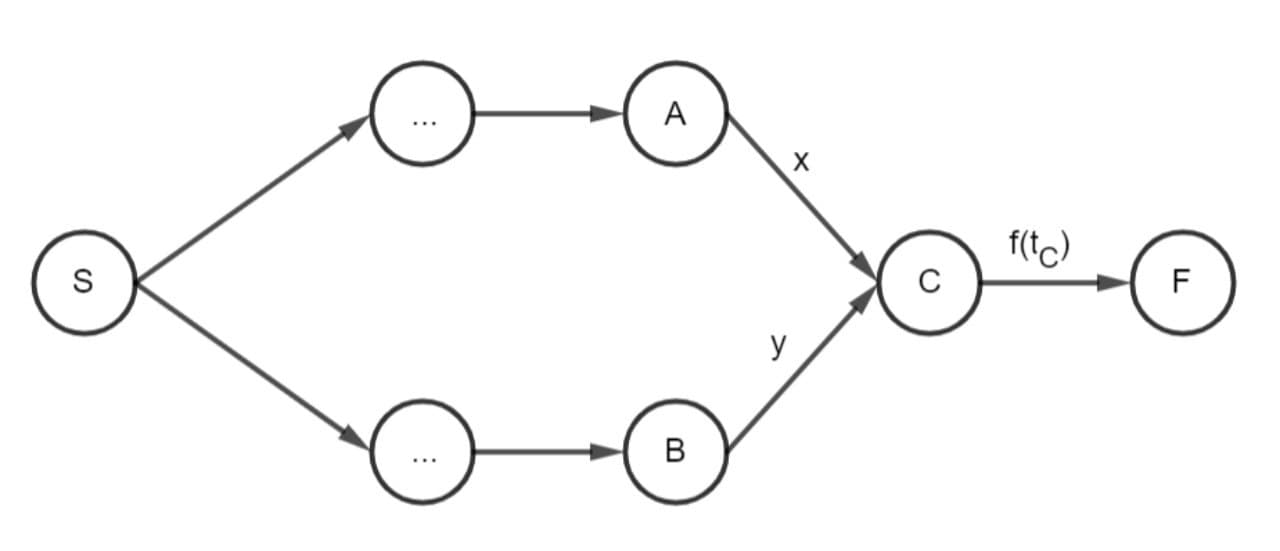
\includegraphics[scale=0.3]{graph_1.jpg}
\end{center}

Без ограничения общности, будем рассматривать часть маршрута P от точки C до F как одно ребро : C-F. Тогда время прохождения этого ребра $\phi(t_C) = \phi_{CF}(t_C)$, где $t_C$ - время старта из точки $C$. Вспомним неравенство прохождения для ребер (см. выше) : $\phi(t_a) \le (t_b - t_a) + \phi(t_b)$, где $\Delta = (t_b - t_a)$

Рассмотрим два маршрута $P : S-...-B-C-F$ и $P': S-...-A-C-F$.
Посчитаем время : $T(P) = t_b + \phi(t_b)$  и $T(P') = t_a + \phi(t_a)$
Используя неравенство, получаем : $T(P') = t_a + \phi(t_a) \le t_a + (t_b - t_a) + \phi(t_b) = T(P)$ Значит маршрут P не является минимальным.

\end{proof}

Понятно, что если неравенство прохождения ребер не выполняется, то модифицированный алгоритм Дейкстры может построить не кратчайший маршрут в терминах временных затрат. Рассмотрим такой пример (рис. \ref{ris:deikstra}):
\begin{align*}
	p_1: & \\
	& t_0 = 0 \\
	& \phi_{AC}(t) = 1  \\
	& \phi_{CB}(t) = 1 + 2 * \mathbb{I} \{t < 1.5\} \\
	p_2: & \\
	& t_0 = 0 \\
	& \phi_{AC}(t) = 2  \\
	& \phi_{CB}(t) = 1 + 2 * \mathbb{I} \{t < 1.5\} 
\end{align*}
Время прохождения пути $p_1$ будет составлять $t_{p_1} = t_0 + \phi_{AC}(t_0) + \phi_{CB}(\phi_{AC}(t_0)) = 1 + 3 = 4 $. Время прохождения пути $p_2$ будет составлять $t_{p_2} = 2 + 1 = 3 $. Очевидно, на путь $p_2$ потребуется меньше времени, чем на путь $p_1$, но алгоритм Дейкстры предложит в качестве решения задачи маршрут $p_1$.

\begin{figure}[H]
	\centering
		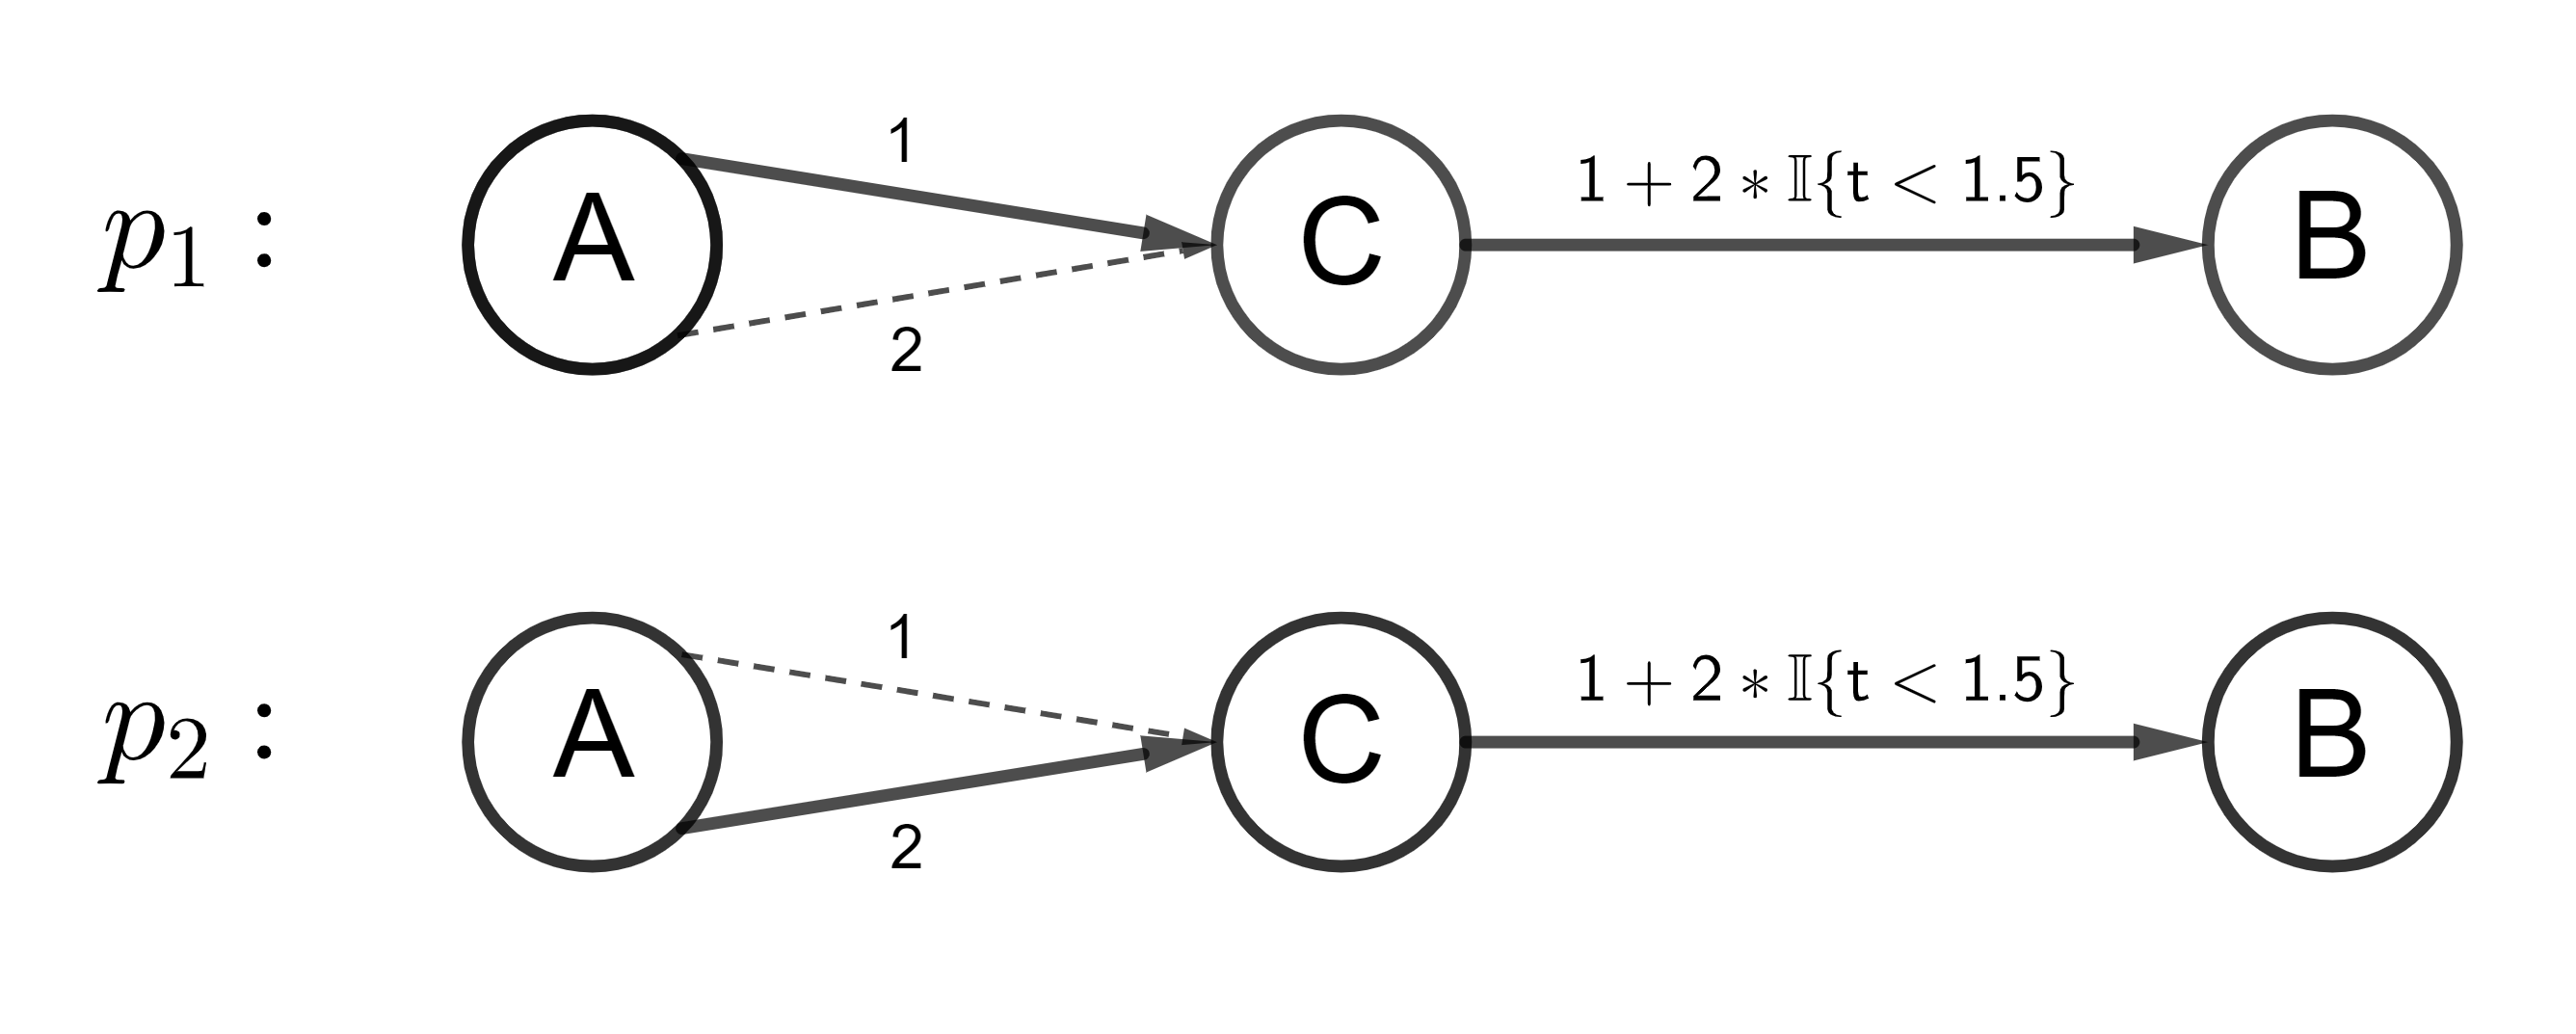
\includegraphics[scale=0.2]{graph_2.png}
	\caption{Пример графа с невыполненным условием неравенства прохождения ребер}
	\label{ris:deikstra}
\end{figure}

Отметим, что наша задача поиска оптимального маршрута сводится к вспомогательной задаче. Правила движения участников и их взаимодействий определяют функции $\phi_e$, $e \in E $. Значения этих функций можно получить путем моделирования движения. Тогда $S_{\phi} = S_M$ и $S = |E|S_M$.

 Неравенство прохождения ребер можно переформулировать так: дорожная сеть обладает условием FIFO --- первый въехавший на дорогу первым ее покидает. Другими словами, если участники не обгоняют друг друга, то путь с минимальными затратами можно найти при помощи алгоритма Дейкстры.

\subsubsection{Применимость модифицированного алгоритма Дейкстры}

%Тут какое-то утверждение про то, что 	Если в модели движения $M$ процесс моделирования движения зависит только от положения участника на ребре, то в $M$ выполняется неравенство прохождения ребер.
Поскольку неравенство прохождения ребер является гарантией того, что модифицированный алгоритм Дейкстры дает оптимальное решение, мы хотели бы исследовать выполнение этого неравенства в интересующих нас моделях движения. Оказывается, что для любой макроскопической модели верно 

\begin{lemma}
	Если в модели движения $M$ процесс моделирования движения зависит только от положения участника на ребре, то в $M$ выполняется неравенство прохождения ребер.
\end{lemma}

\begin{proof}
Докажем от противного. Рассмотрим одного участника и его копию, которая могла двигаться в другое время по дургому ребру. И участник, и копия зависят от движений других участников, но друг на друга не влияют. Итак, пусть участник въезжает на ребро $e$ в разные моменты времени $t_1$ и $t_2$, $t_2 > t_1$ с ребер $e_1$ и $e_2$ соответственно. Пусть $\chi(t)$~-- часть пройденного ребра $e$. Предположим, что $\phi_e(t_1) > (t_2-t_1) + \phi_e(t_2)$, тогда в какой-то момент времени $t$ $\chi_1(t) = \chi_2(t) \; \Rightarrow  $

\end{proof}


%Потом говортся, что макроскопические все такие хорошие и супер--пупер


В микроскопических моделях условия выполнимости неравенства не найдены, а как мы уже выяснили на примере (см. рис. \ref{ris:deikstra}), модифицированный алгоритм Дейкстры может выдать не оптимальное решение задачи, если неравенство прохождения ребер не выполнено. Беря во внимание этот факт, мы предлагаем не отказываться от применения алгоритма и к микроскопическим моделям. Для них можно посчитать погрешность алгоритма.

Обратимся к описанной нами микроскопической модели (см. рис. \ref{ris:micro_diag}) и рассмотрим случай, когда участник мог бы <<обогнать>> самого себя, если бы начал движение позднее. Опишем худший случай в нашей модели на бесконечном ребре. Участник оказывается на расстоянии $d \approx 0$ до лидера и теряет свою скорость до $v_{min}$. Пусть лидер и участник со сдвигом по времени двигаются со скоростями $v_{max}$ на расстоянии $l+\varepsilon, \: \varepsilon > 0$ друг от друга и они не меняют своих скоростей. В таком случае участнику, близкому к лидеру, нужно отдалиться на безопасное расстояние $D$ за $t_1 = \frac{D}{v_{max}-v_{min}}$ и разогнаться до скорости $v_{max}$ за $t_2 = \frac{v_{max}-v_{min}}{a}$. За это время $t = t_1 + t_2$ участник со сдвигом преодолеет расстояние $s = v_{max}t$. Расстояние между участником и его копией через время $t$ составит
$$\Delta s =  D - l + \frac{\left(v_{max}-v_{min}\right)^2}{2a}.$$
%\newpage
%\section*{Устойчивость нашего решения}



\newpage
\section*{Практические результаты}



\newpage
\section*{Заключение}

В ходе написания дипломной работы были совершены следующие шаги:

 \begin{itemize}
	\item Предложена автоматная форма определения модели движения АТС.
	\item Разработан и реализован алгоритм симуляции движения АТС в соответствии с заданной моделью движения.
	\item Сформулировано необходимое условие, при котором модифицированный алгоритм Дейкстры приводит к нахождению оптимального решения.
	\item Показано, что для модели следования за лидером возможно отклонение найденного решения от оптимального.
\end{itemize}

Исследование может иметь продолжение в различных направлениях: разработки более сложной и приближенной к реальности модели движения; рассмотрение случая, когда добавленный участник влияет на движение всех остальных АТС; проверки устойчивости найденного решения; поиска аналогий задачи или подзадач в разных областях математики.
    \newpage
\begin{thebibliography}{0}
	
	\addcontentsline{toc}{section}{Литература}
	
	\bibitem{hydro_1} \textit{Lighthill M. J., Whitham G. B.} On kinematic waves: II. Theory of traffic
	flow on long crowded roads // Proc. R. Soc. London, Ser. A. 1955.
	V. 229. P. 281–345.
	
	\bibitem{hydro_2} \textit{Richards P. I.} Shock Waves on the Highway // Oper. Res. 1956. V. 4.
	P. 42–51.
	
	\bibitem{Tanaka} \textit{Иносэ Х., Хамада Т.} Управление дорожным движением. М.: Транс-
	порт, 1983.
	
	\bibitem{Newwell} \textit{Newell G. F.} Nonlinear effects in the dynamics of car – following //
	Oper. Res. 1961. V. 9. P. 209–229.
	
	\bibitem{book} \textit{А.\,И.~Гасников} ``Введение в математическое моделирование транспортных потоков'' --- Издательство МЦНМО --- 2013. --- 427 с.
	
	\bibitem{automat_baza} \textit{Nagel K., Schreckenberg M.} A cellular automation model for freeway
	traffic // Phys. I France. 1992. V. 2. P. 2221–2229.
	
	\bibitem{automat_phyz} \textit{Chowdhury D., Santen L., Schadschneider A.} Statistical physics of vehicular
	traffic and some related systems // Phys. Rep. 2000. V. 329.
	P. 199–329.
	
	\bibitem{automat_jam} \textit{Nagatani T.} The physics of traffic jams // Reports on Progress in Physics.
	2002. V. 65. P. 1331–1386.
	
\end{thebibliography} 

\end{document}